\documentclass[]{IEEEtran}
% some very useful LaTeX packages include:
%\usepackage{cite}      
\usepackage{graphicx}   
\usepackage{subfigure} 
\usepackage{url}       
\usepackage{amsmath}    
\usepackage{caption2}
% Your document starts here!
\begin{document}

% Define document title and author
	\title{Weekly Report}
	\author{Adviser: Prof. Yang Wen \\Student: Cheng Wensheng\\ Period: 2018.7.1-7.8
	}
	\markboth{Visual Information Processing Group}{}
	\maketitle

% Write abstract here
\begin{abstract}
	This week I mainly put my effort on reading Apple's paper and WGAN, then made a report on group meeting. 
\end{abstract}

% Each section begins with a \section{title} command
\section{Paper reading}
	% \PARstart{}{} creates a tall first letter for this first paragraph
	\PARstart{I}{n} this paper, they propose Simulated+Unsupervised
	(S+U) learning, where the goal is to improve the realism
	of synthetic images from a simulator using unlabeled
	real data. The improved realism enables the training
	of better machine learning models on large datasets
	without any data collection or human annotation effort.
	In addition to adding realism, S+U learning should preserve annotation information for training of machine
	learning models. Moreover, since machine learning
	models can be sensitive to artifacts in the synthetic data, S+U learning should generate images without artifacts.

	They develop a method for S+U learning, which they
	term SimGAN, that refines synthetic images from a simulator using a neural network which called ‘refiner
	network’.
	In conclusion, the following points show our main contributions:
	\begin{itemize}
		\item They propose S+U learning that uses unlabeled real data to refine the synthetic images.
		\item They train a refiner network to add realism to synthetic images using a combination of an adversarial
		loss and a self-regularization loss.
		\item They make several key modifications to the GAN
		training framework to stabilize training and prevent
		the refiner network from producing artifacts.
		\item They present qualitative, quantitative, and user study experiments showing that the proposed framework significantly improves the realism of the simulator output. We achieve state-of-the-art results, without any human annotation effort, by training deep neural networks on the refined output images.
	\end{itemize}
	
	Fig.~\ref{fig:fw} is the overview of SimGAN. Fig.~\ref{fig:rt} the example refined test images for the NYU hand pose dataset.
	

% Main Part

\newpage
\begin{figure}[!hbt]
%		 Center the figure.
		\vspace{1.7cm}
%		\hspace{50cm}
		\begin{center}
			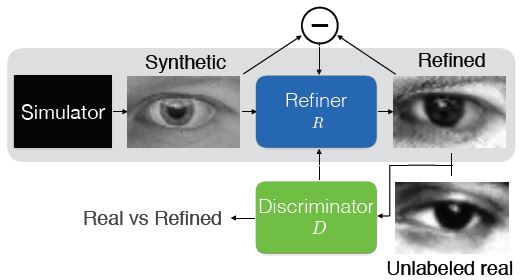
\includegraphics[width=\columnwidth]{fw}
				%		 Create a subtitle for the figure.
			\caption{Overview of SimGAN.}
			\label{fig:fw}
		    \hspace{0.5cm}
			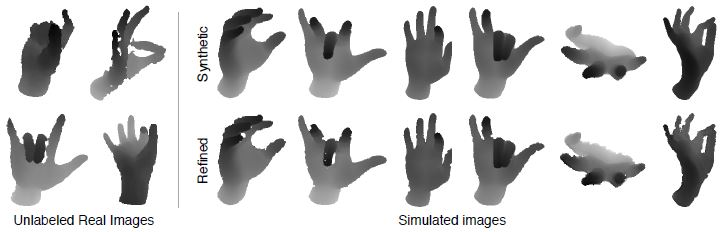
\includegraphics[width=\columnwidth]{rs}
				%Create a subtitle for the figure.
			\caption{Example refined test images for the NYU hand pose dataset}
			\label{fig:rt}
		\end{center}
	\end{figure}

% Now we need a bibliography:
%\begin{thebibliography}{5}
%
%	%Each item starts with a \bibitem{reference} command and the details thereafter.
%	\bibitem{HOP96} % Transaction paper
%	J.~Hagenauer, E.~Offer, and L.~Papke. Iterative decoding of binary block
%	and convolutional codes. {\em IEEE Trans. Inform. Theory},
%	vol.~42, no.~2, pp.~429–-445, Mar. 1996.
%
%	\bibitem{MJH06} % Conference paper
%	T.~Mayer, H.~Jenkac, and J.~Hagenauer. Turbo base-station cooperation for intercell interference cancellation. {\em IEEE Int. Conf. Commun. (ICC)}, Istanbul, Turkey, pp.~356--361, June 2006.
%
%	\bibitem{Proakis} % Book
%	J.~G.~Proakis. {\em Digital Communications}. McGraw-Hill Book Co.,
%	New York, USA, 3rd edition, 1995.
%
%	\bibitem{talk} % Web document
%	F.~R.~Kschischang. Giving a talk: Guidelines for the Preparation and Presentation of Technical Seminars.
%	\url{http://www.comm.toronto.edu/frank/guide/guide.pdf}.
%
%	\bibitem{5}
%	IEEE Transactions \LaTeX and Microsoft Word Style Files.
%	\url{http://www.ieee.org/web/publications/authors/transjnl/index.html}
%
%\end{thebibliography}

% Your document ends here!
\end{document}